% !TEX root = ../neurosciences-barrels.tex

\section{Results}
\label{sec-results}

Starting from tangential slices stained for cytochrome oxidase, the reconstructed 2-D barrel map can be obtained in a few clicks by using the provided GUI. The whole procedure takes 7-9 minutes including 3-5 minutes of computation that do not require the intervention of the user. The same process using traditional manual methods (with the help of a raster graphics editor such as Adobe Photoshop) takes, for a well-trained person, 16 to 28 minutes. Most importantly, our automated approach prevents user dependent variability in the obtained barrel map.
In order to assess the accuracy of our registration method we first carried out histological control experiments, and then used VSD imaging to functionally evaluate the precision of the barrel map obtained following the full reconstruction procedure.


%%%%%%%%%%%%%%%%%%%%%%%%%%%%%%%%%%%%%%%%%%%%%%%%%%%
%%%%%%%%%%%%%%%%%%%%%%%%%%%%%%%%%%%%%%%%%%%%%%%%%%%
%%%%%%%%%%%%%%%%%%%%%%%%%%%%%%%%%%%%%%%%%%%%%%%%%%%
\subsection{Histological Validation of the Registration Method}

In order to assess the efficiency of our registration method based on automated blood vessel detection and robust ICP, we perpendicularly inserted DiI coated electrodes in the barrel cortex of urethane anesthetized mice ($n=5$ experiments, 3 to 6 electrode penetrations per experiments), before processing the brain for histological staining of the cytochrome oxidase following our standard procedures. 
%
% The DiI stain being fluorescent, it is not visible on cytochrome oxidase staining images taken under transmitted light, and therefore does not interfere with our registration method (Figure~\ref{fig-histo-validation}). 
The electrodes being flat, they did not leave any round or elliptic white marks in the tissue and therefore did not interfere with our registration method (Figure~\ref{fig-histo-validation}).
%
Because the penetration of DiI coated electrodes was perpendicular to the cortical surface, the DiI staining  should appear aligned on consecutive cortical sections following proper registration of the slices. In order to control this alignment, the location of DiI spots was reported for each slice on the final fused barrel map image for each section (Figure~\ref{fig-histo-validation}C).  
%
The calculated mean distance between DiI spots from the same electrode penetration ($34.41\pm18.93$~$\mu$m, mean $\pm$ SD, $n=5$) revealed the subcolumnar resolution of our registration method. 
%
These control experiments were further used to evaluate the eventual shrinkage of the cortical tissue due to brain fixation and histological procedures. The distances of 250~$\mu$m and 500~$\mu$m separating the electrode penetration sites in vivo, were compared to the distances measured between DiI spots on the slices following histological procedures. Over our 5 control experiments, the observed tissue shrinkage within the x-y plane was minimal ($<1.5\%$).


\begin{figure*}[!ht]
\centering
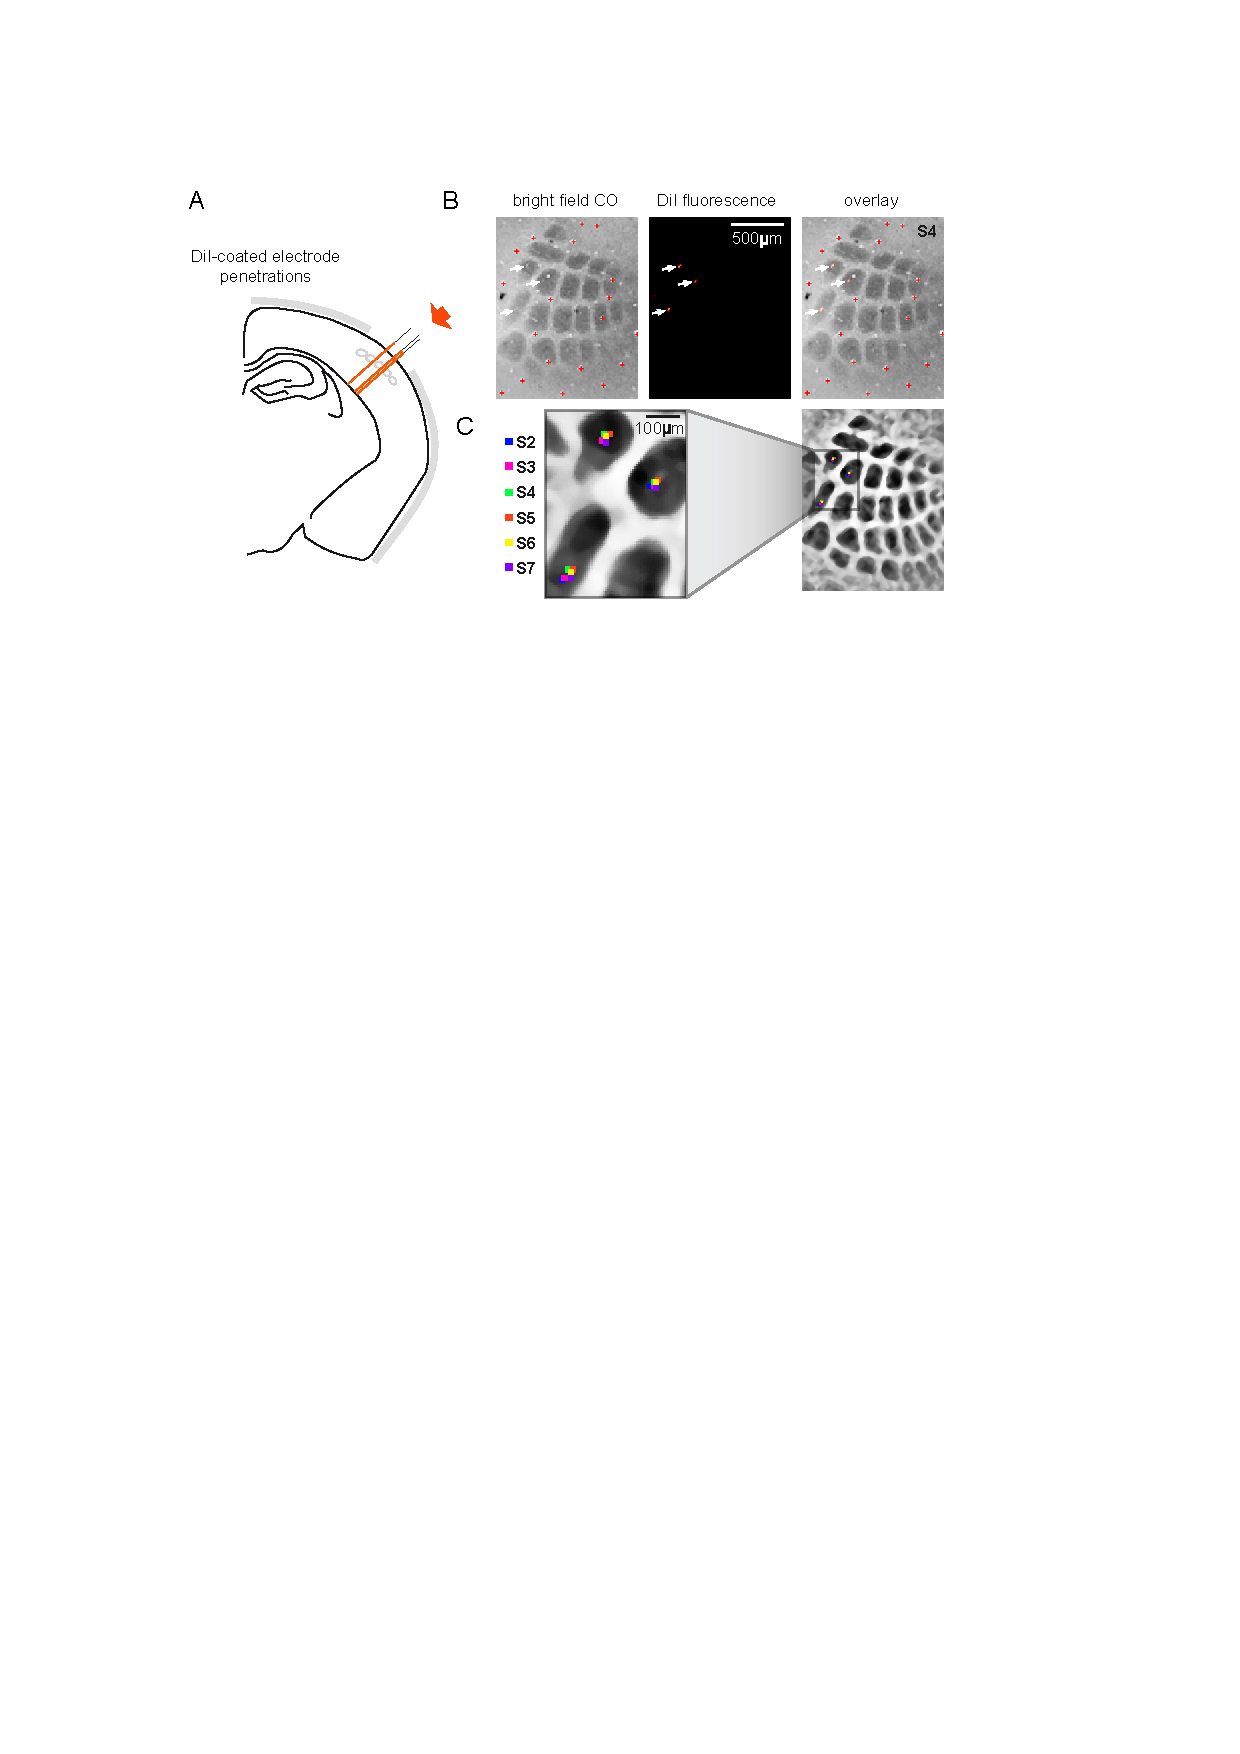
\includegraphics[width=140mm]{images/Perronnet-Figure4}
\caption{
	\textbf{Histological validation of the registration method.} \\
	% 
	\textbf{A.} Drawing of a coronal section of the left hemisphere of the mouse brain illustrating the penetration sites of DiI-coated electrodes. 
	% 
	\textbf{B.} The DiI fluorescent staining (middle image) does not interfere with the process of blood vessel detection used on bright field images (left), as shown by the absence of detected spots on the DiI stain (right), arrowheads indicate the DiI stained spots corresponding to electrode tracks. 
	%
	\textbf{C.} Following the registration of the slices 2 to 7, we observe a good overlap of DiI spots, indicative of the accuracy of our registration method.
}
\label{fig-histo-validation}  
\end{figure*}


%%%%%%%%%%%%%%%%%%%%%%%%%%%%%%%%%%%%%%%%%%%%%%%%%%%
%%%%%%%%%%%%%%%%%%%%%%%%%%%%%%%%%%%%%%%%%%%%%%%%%%%
%%%%%%%%%%%%%%%%%%%%%%%%%%%%%%%%%%%%%%%%%%%%%%%%%%%
\subsection{Assessment of the barrel map reconstruction tool using VSDI of cortical responses to individual whisker deflections}

To finally validate our 2-D barrel map reconstruction method, we confronted its resulting map with the functional organization of the barrel cortex established in vivo by real time imaging of cortical responses to individual whisker deflections under urethane anesthesia ($n=4$ experiments). Using a mechanical multi-whisker stimulator~\cite{Jacob10}, we deflected independently the 24 principal whiskers in a pseudo random order, and imaged the evoked cortical responses in the contralateral barrel cortex using the VSD RH1691. 
Figure~\ref{fig-func-validation} illustrates the results obtained from one experiment.
As previously reported in similar conditions~\cite{ferezou_2006}, the earliest responses to whisker deflections were localized to the corresponding barrel-related columns (Figure 5A). 
% The underlying histological arrangement of the barrels in layer 4 was subsequently determined following our proposed semi-automated workflow and realigned to the functional images using the superficial blood vessels as landmarks (Figure 2). 
%
When reporting the 90\% contours of the early cortical responses onto the aligned barrel map, we observe a good anatomo-functional match (Figure~\ref{fig-func-validation}B).
%
To quantify this match, the distance between the centroid of the anatomically defined barrels and the centroid of the early VSD response (area above a 90\% threshold) was measured (Figure~\ref{fig-func-validation}C). The mean centroid-centroid distance over the 4 control experiments for all the barrels is $60.5\pm21.2$~$\mu$m (34.8--116.5~$\mu$m range across the barrel field). We observed slightly higher values for the columns located at the border of the map which might result from the curvature of the cortex, the  maxima of cortical responses were located within the corresponding barrel area in the majority of cases (86.55\%), attesting to the accuracy of the method.


% REMOVED
% Indeed, the anatomically defined barrels are covered at 67.3\% and 73.7\% (in average, for the first and second experiment, respectively) by the peak of the early functional responses (area above a 90\% threshold). Although for the barrels located on the A and E rows, the early cortical responses appear a little shifted relative to the center of their corresponding barrels due to the curvature of the cortex, the maxima of cortical responses were located within the corresponding barrel area in the majority of cases (83.3\% and 95.6\%, respectively), attesting for the accuracy of the method.


% , attesting for the accuracy of our method.  Note that for the barrels located on the A and E rows, the early cortical responses appear a little shifted relative to the center of their corresponding barrels due to the curvature of the cortex.



\begin{figure}[h!]
\centering
	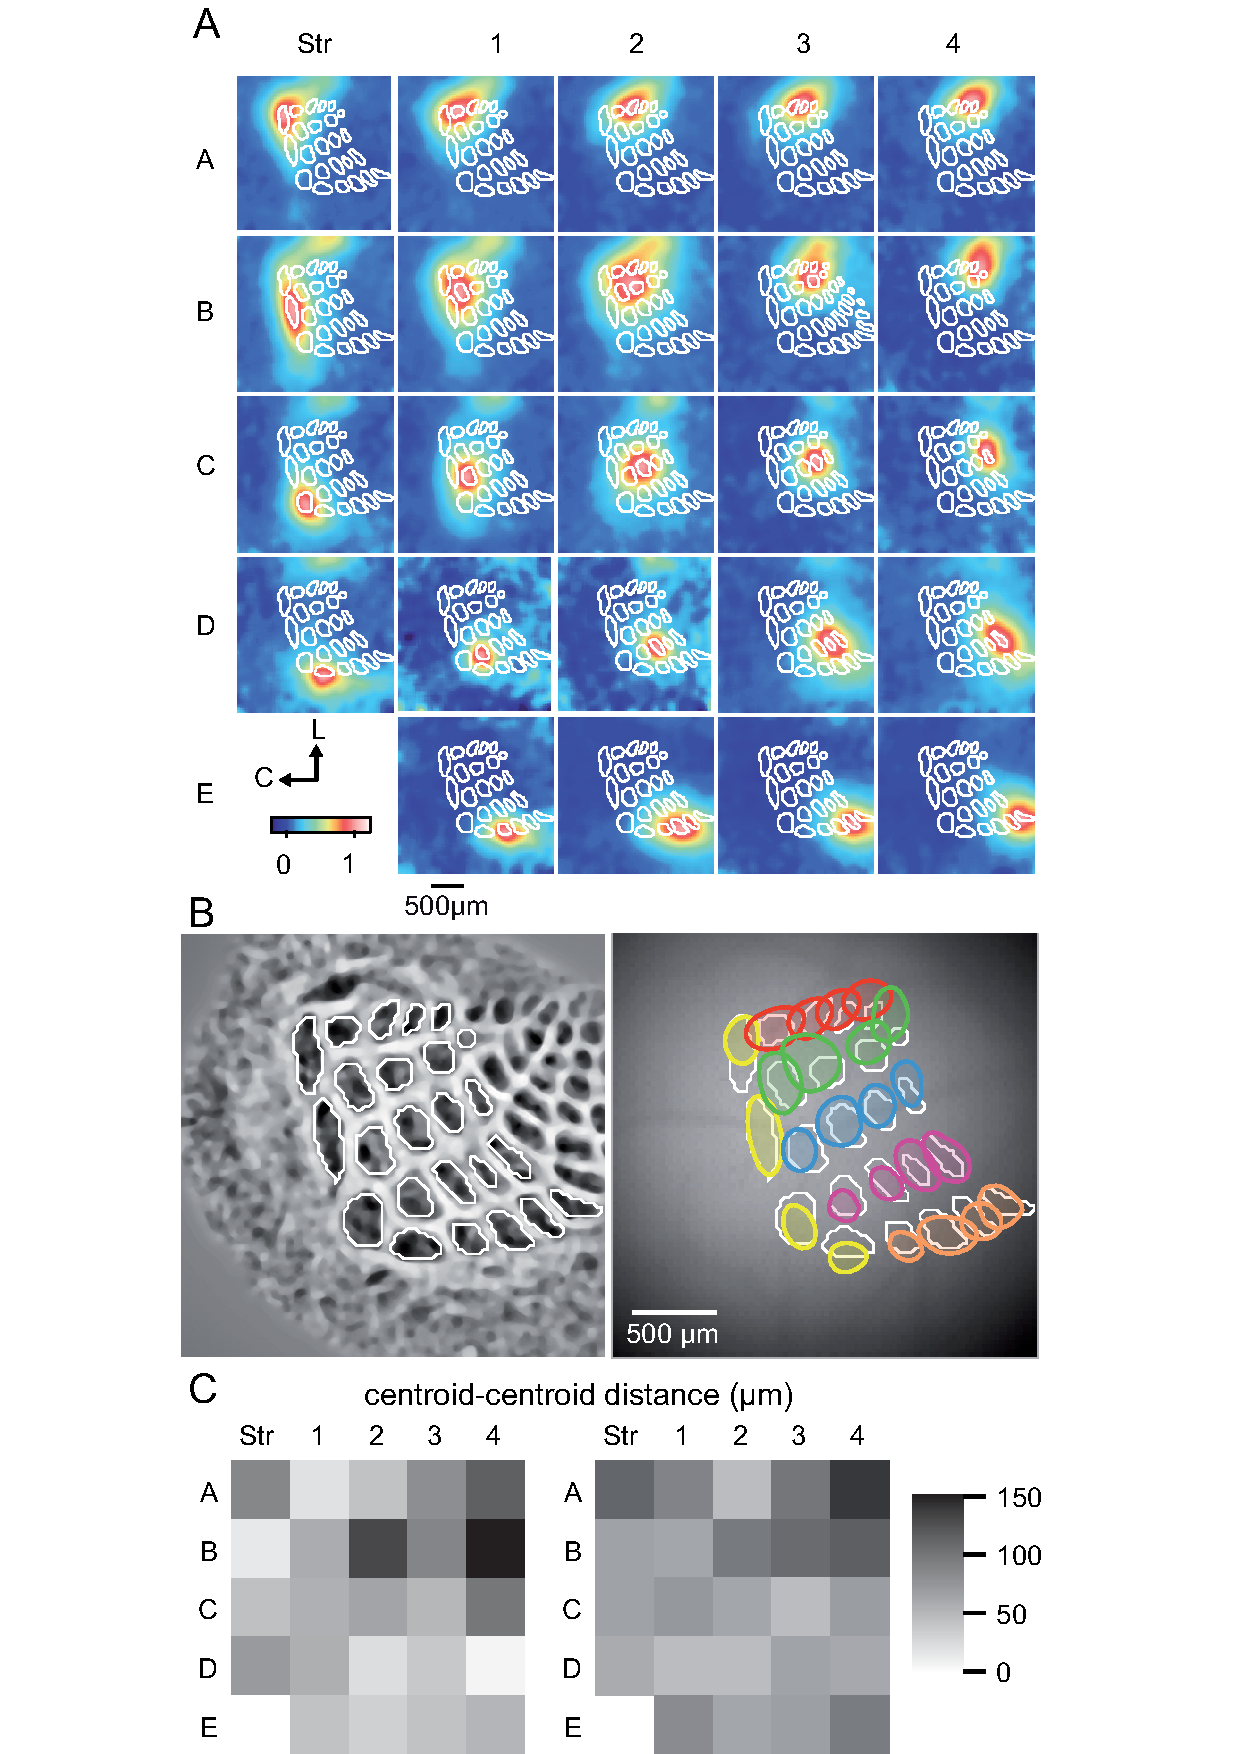
\includegraphics[width=80mm]{images/Perronnet-Figure5} % WAS 88mm
\caption{
	\textbf{Functional validation of the registration method.}
	%
	\textbf{A.} Cortical responses evoked by individual deflections of the 24 principal vibrissae in a urethane anesthetized mouse were imaged using the VSD RH1691. For each whisker, the early cortical response is shown (data averaged from 4 to 18 ms post stimulation time and 40 trials, Gaussian filtered ($5 \times 5$ pxls), and normalized), together with the aligned barrel map obtained from our reconstruction method (white lines). 
	%
	\textbf{B.} The barrel map was extracted from the fused barrel field image (left) and overlaid on the VSD reference image (right) together with the early response locations (90\% contours of the early responses (in A) are shown in colors) obtained for each whisker. 
	%
	\textbf{C.} The distance between the centroid of the barrel area and the centroid of the early cortical response (as illustrated in B) was computed, column by column, for the experiment illustrated in A-B (left), and in average for all the control experiments ($n = 4)$.
}
\label{fig-func-validation}  
\end{figure}


